%oliwis aqui estoy YO!!!
%=========================================================
\chapter{Concepto}
%\section{Concepto}

		\section{Título:} Yolotl.
		%---------------------------------------------------------
		\section{Diseñadoras:} Hernández Bautista 				Yasmine Pilar,  Márquez Hernández Karla Rocío..
%---------------------------------------------------------
    	\section{Género:} Plataforma. Aventura.
    	%---------------------------------------------------------
   		\section{Plataforma:} Dispositivos móviles Android.    			\begin{itemize}
   		
			\item Dispositivo de prueba 1:
   		\begin{itemize}
   			\item Versión 5.2
   			\item Modelo Huawei TAG-L13
   			\item CPU MediaTek MT6753 1,50 GHz
   			\item IPS TFT 16M colors 720 x 1280 px (5,00) 294 ppi
   			\item RAM 2GB
   			
   		\end{itemize}
   		
   		\item Dispositivo de prueba 2:
   		\begin{itemize}
   			\item Versión 7.0
   			\item Modelo ASUS X008DC
   			\item CPU MediaTek Quad Core Processor
   			\item GPU Mali T720
   			\item RAM 3GB LPDDR3
   			\item PANEL 5.2-inch
   			HD(1280 x 720) IPS display 
   			75 por ciento screen-to-body ratio
   			400nits brightness 
   		\end{itemize}   		
   		
   		\end{itemize}
%---------------------------------------------------------   
    	\section{Versión:} V03.18/10/17
    	%---------------------------------------------------------
   		\section{Sinopsis de jugabilidad:} 
Haciendo uso de la interfaz gráfica y la pantalla táctil del dispositivo móvil, el jugador controlará a Malinalli pudiendo moverse hacia la izquierda o la derecha, realizar un salto o un doble salto, o disparar tonalli (Ver Figura\ref{fig:GUI}). Estas habilidades le permitirán al jugador superar los diferentes obstáculos, plataformas y enemigos a lo largo de los diez niveles que componen al juego.
\\
\par
Los niveles del dos al nueve están compuestos por dos etapas una de plataformas, en donde el jugador superar obstáculos y enemigos comunes, y otra de batalla de jefe en donde el jugador deberá derrotar al Dios guardián del nivel para avanzar al siguiente nivel. En el nivel uno el jugador superará dos zonas: la primera zona consistirá en dialogar con ciudadanos y en la segunda zona deberá de superar diferentes obstáculos. En el nivel diez, el jugador deberá enfrentarse al jefe final.
   		
   		
 

\begin{figure}
				\centering
				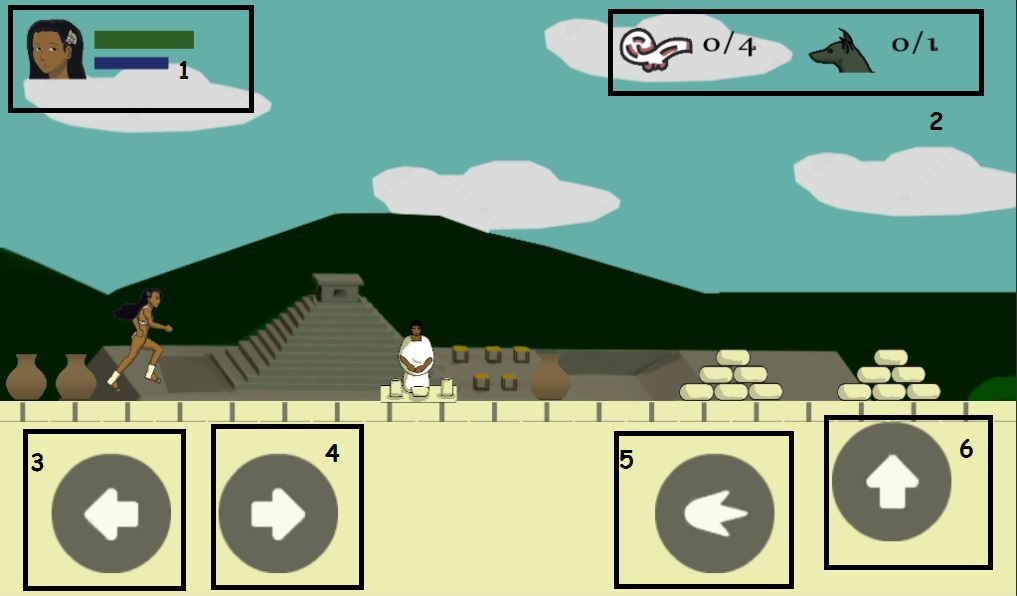
\includegraphics[height=0.3 \textheight]{Imagenes/ControlCorrerDer}
				\caption{1 Información del personaje jugable, barra verde indicador de la cantidad de vida, barra azul cantidad de tonalli. 2 Objetivos del nivel o información útil. 3 Botón moverse izquierda. 4 Botón moverse derecha. 5 Botón disparar tonalli. 6 Botón saltar.}
				\label{fig:GUI}
\end{figure}

%---------------------------------------------------------  		
    	\section{Sinopsis de contenido:} 
La historia se centra en Malinalli Tenelpan, una joven esclava que desea revivir a su padre, y el dios Xólotl, un Dios exiliado que se ha ofrecido a revivir al padre de Malinalli a cambio de su ayuda, cuyo objetivo es restaurar el orden de la jerarquía divina luego de que Tezcatlipoca y Quetzalcóatl la sumergieran en un espiral de caos con sus múltiples batallas por el liderazgo de los dioses. 
\\
\par
Para cumplir sus objetivos, Malinalli y Xólotl bajaran al Mictlan. Ahí enfrentaran a los guardianes del Mictlan, que son Dioses de gran poder cuyas habilidades se relacionan con un aspecto de la muerte. Siendo el último a vencer el señor y gobernante del Mictlan: el dios Mictlantecuhtli.
\\
\par
A lo largo de la narrativa, el jugador irá descubriendo el pasado de los dos protagonistas, de igual forma aprenderá sobre el funcionamiento del mundo de los dioses, sus reglas, su jerarquía y sus integrantes.
%---------------------------------------------------------
	\section{Categoría:}
A continuación se presentará una tabla comparativa que muestra la diferentes juegos que, por sus mecánicas o temática, pueden ser considerados como productos similares a Yolotl.
\begin{itemize}
	\item Guacamelee!!
	\begin{itemize}
		\item Microsoft Windows, OS X, Linux, PlayStation 3, PlayStation 4, PlayStation Vita, Wii U, Xbox 360, Xbox One.
		\item 103.12 a 206.03 (dependiendo de la plataforma)
		\item Plataforma, Metrodvania.
		\item Personas mayores de 10 años
		\item Diferencia: No es contexto de caracter histórico, no es móvil.
	\end{itemize}

\item Never Alone
\begin{itemize}
	\item Linux, Microsoft Windows, OS X, PlayStation 3, PlayStation 4, Wii U, Xbox One, iOS, Android.
	\item 150.00 a 89.00 (dependiendo de la plataforma)
	\item Plataforma, puzzle.
	\item Personas mayores de 10 años.
	\item Diferencia: No cuenta con estatus de vida o elementos de ataque del personaje, no es móvil.
\end{itemize}


\item Valiant Hearts
\begin{itemize}
	\item Microsoft Windows, Xbox One, PlayStation 4, PlayStation 3, wiistation 360, Android y iOS.
	\item 285.00
	\item Juego de Lógica. 
	\item Personas mayores de 13 años.
	\item Diferencia: No es un juego de plataforma, no es móvil.
\end{itemize}


\item Olympia rising.
\begin{itemize}
	\item Wii U.
	\item 95.11
	\item Acción y aventura.
	\item Mayores de 10 años.
	\item Diferencia: No es un juego móvil.
\end{itemize}


\item Jotun: Valhalla Edition.
\begin{itemize}
	\item PlayStation 4, Xbox One, Wii U, Microsoft Windows, GNU/Linux, Mac OS.
	\item 150.00
	\item Acción Aventura.
	\item Personas mayores de 13 años.
	\item Diferencia: No es un juego móvil, no es de plataforma.
\end{itemize}

\end{itemize}
%---------------------------------------------------------
	\section{Licencia:}
Atribución-NoComercial-CompartirIgual 
CC BY-NC-SA
%---------------------------------------------------------
	\section{Mecánica:}
	Haciendo uso de la pantalla touch del teléfono móvil y de una interfaz gráfica, el jugador controlará a Malinalli, siendo ella el personaje jugable durante todo el juego, salvo en un nivel en donde tanto ella como Xólotl serán los personajes jugables.   El jugador hará que Malinalli pueda moverse de izquierda a derecha, realice un salto o un salto doble, ataque con tonalli o dialogue con otros personajes.
\\
\par
En total el jugador deberá de pasar 10 niveles para terminar el juego. Cada nivel está diseñado para que el jugador tenga que superar diferentes plataformas y derrotar enemigos (enemigos comunes y jefes de nivel). Algunos niveles están más orientados a la superación de obstáculos, otros a la exploración y algunos al combate, siendo la constante entre todos (salvo el nivel introductorio), el tener que derrotar a un jefe al final del nivel.
\\
\par
La GUI contendrá cuatro botones(ver  figura \ref{fig:GUI}): uno para moverse a la izquierda, otro para moverse a la derecha, otro más para saltar y uno para disparar tonalli. En la parte superior de la pantalla habrá dos iconos uno para indicar la cantidad de vida de Malinalli y otro para la cantidad de tonalli para disparar. La cantidad de tonalli disminuirá con cada ataque que el jugador efectué y cuando éste llegué a cero, el jugador podrá disparar hasta después de que se reestablezca la barra de tonalli o si logra obtener el ítem Flor de vainilla(ver figura \ref{fig:UsoTonalli} ). Cuando un disparo de tonalli colisiona con un enemigo, éste desaparece si es un enemigo común o se le infringe una cantidad de daño determinada en caso de que sea un jefe (Ver figura \ref{fig:InterEnemigo}). La vida de Malinalli disminuirá si recibe ataques de los enemigos o si colisiona con alguno (ver figura \ref{fig:Danio}). Cada enemigo tiene una cantidad de daño asignada, siendo los jefes de cada nivel los enemigos con mayor capacidad de infringir daño. La partida acabará si la vida de Malinalli llega a cero. El jugador podrá recuperar vida con el ítem Grano de Cacao.

\begin{figure}
				\centering
				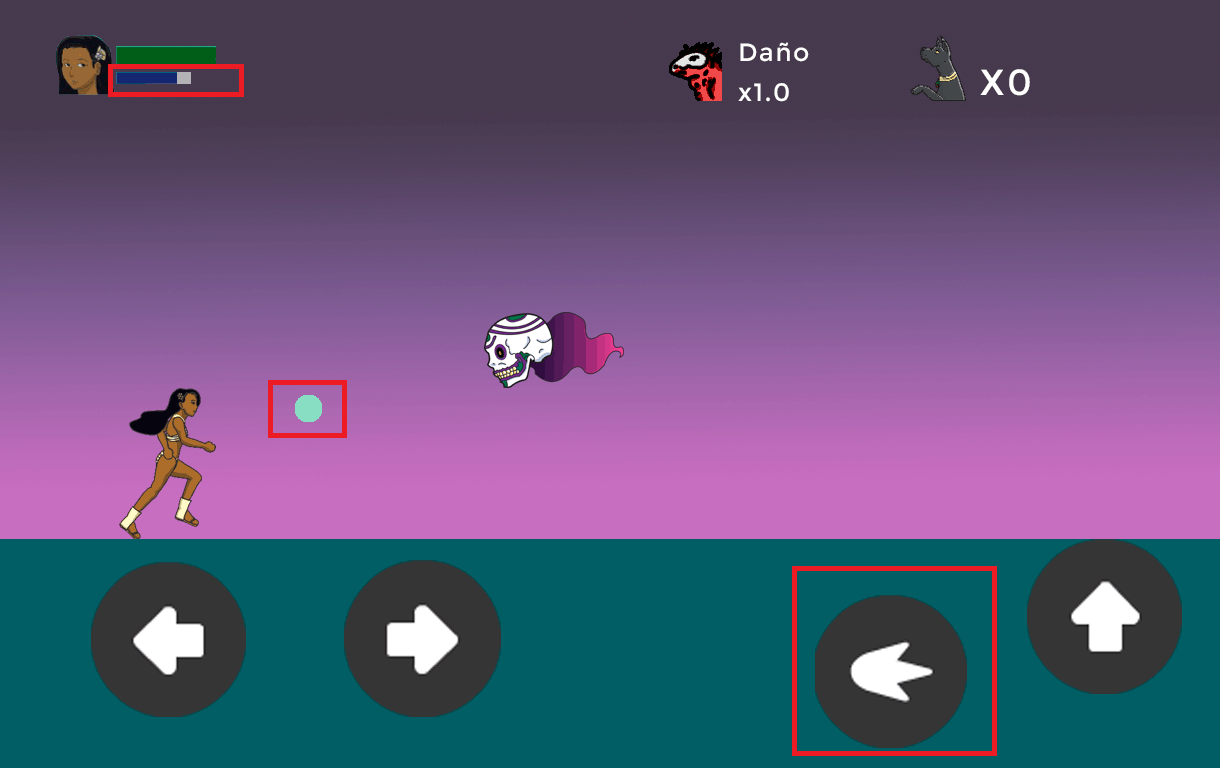
\includegraphics[height=0.3 \textheight]{Imagenes/nivel02_tonalli}
				\caption{Cuando el jugador dispara se consume una fracción de la barra de tonalli.}
				\label{fig:UsoTonalli}
\end{figure}

	\begin{figure}
  \centering
  \subfigure[Disparo de tonalli.]{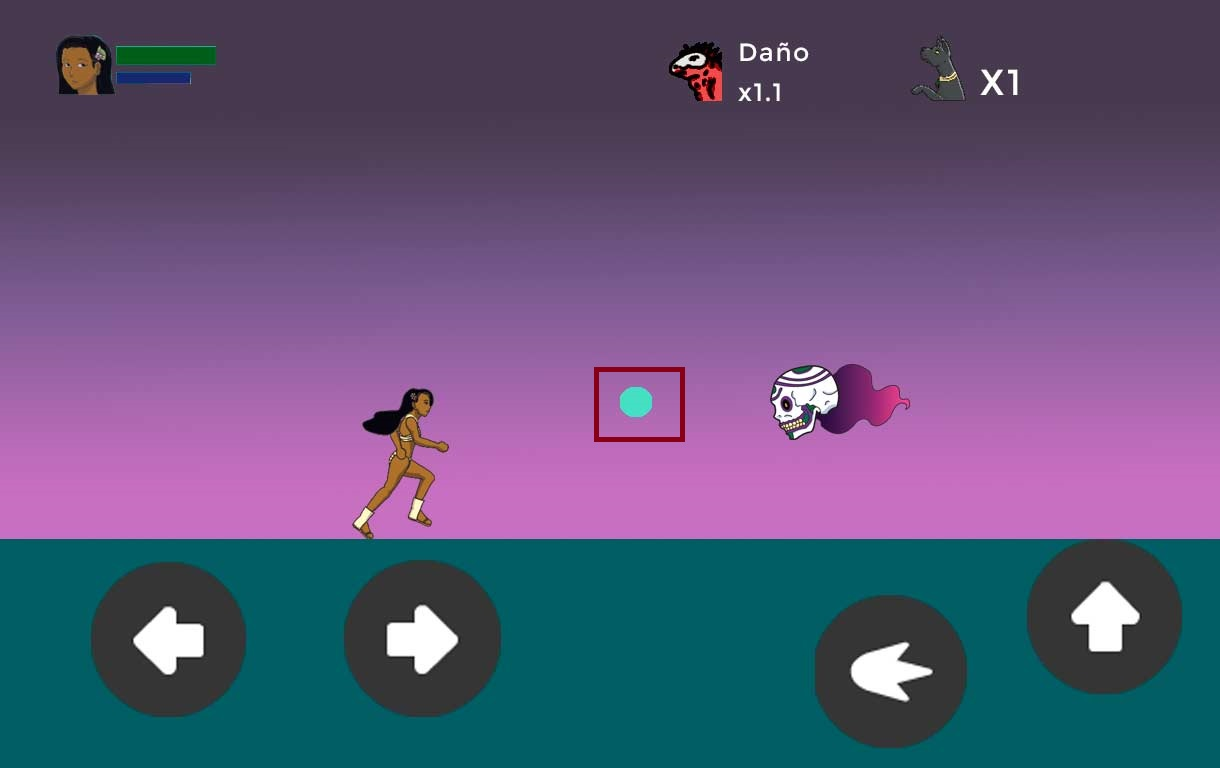
\includegraphics[width=0.45 \textwidth]{Imagenes/PantallaInteraccionEnemigo}}
   \subfigure[Colisión disparo de tonalli con enemigo común.]{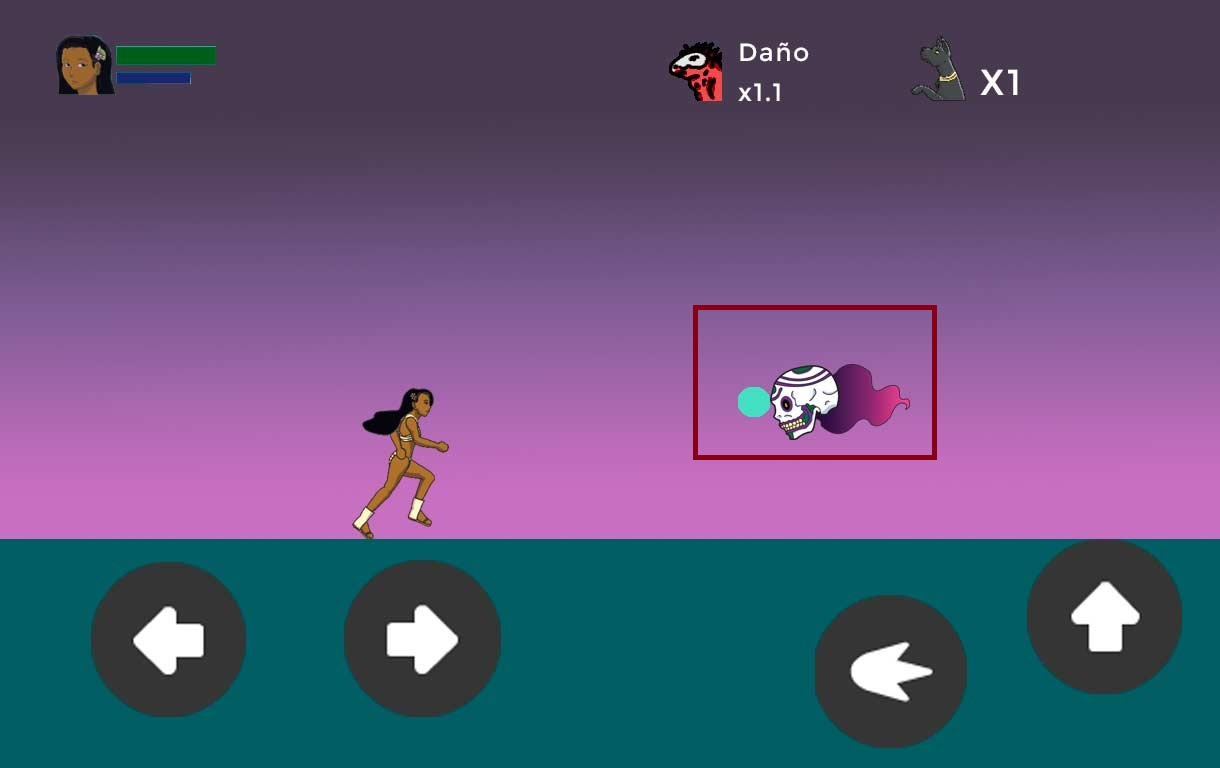
\includegraphics[width=0.3 \textwidth]{Imagenes/PantallaInteraccionEnemigo02}}
   \subfigure[Destrucción del enemigo y el disparo de tonalli.]{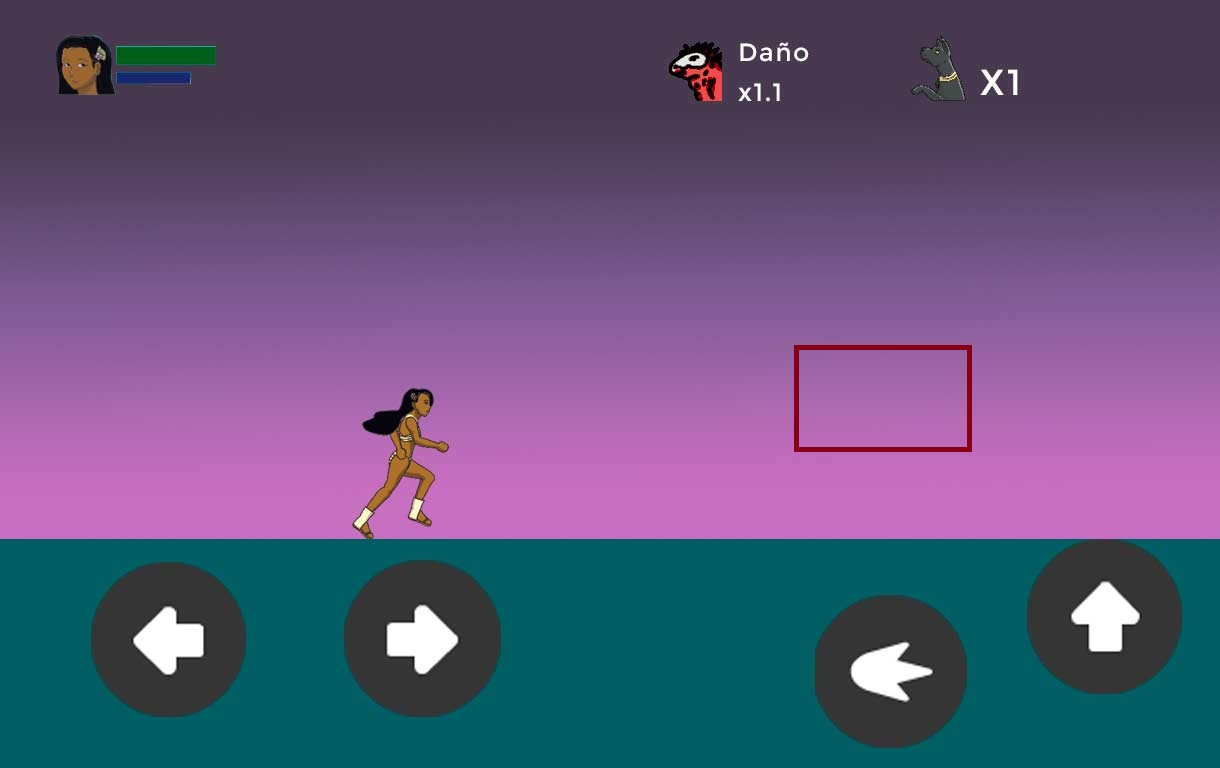
\includegraphics[width=0.3 \textwidth]{Imagenes/PantallaInteraccionEnemigo03}}
  \caption{Interacción entre el enemigo y el disparo de tonallia}
  \label{fig:InterEnemigo}
\end{figure} 

\begin{figure}
				\centering
				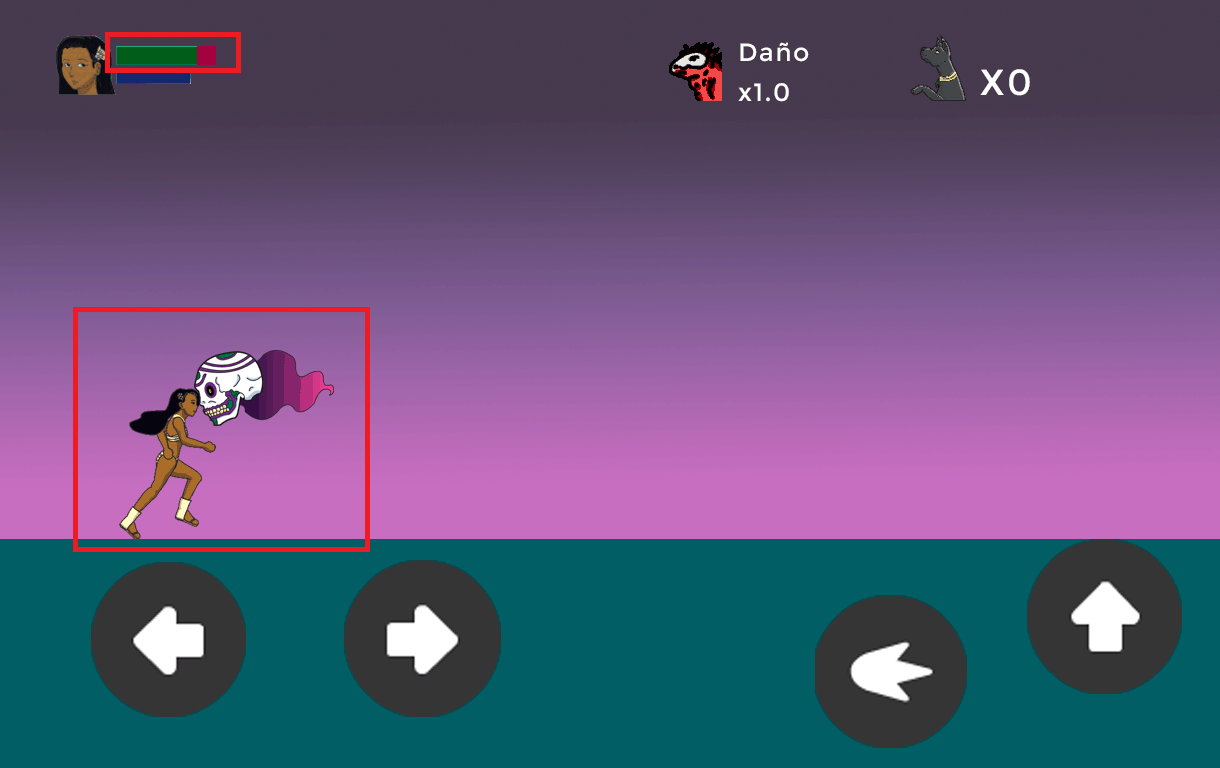
\includegraphics[height=0.3 \textheight]{Imagenes/nivel02_danio}
				\caption{Cuando el jugador colisiona con un enemigo el personaje jugable recibe daño y su cantidad de  vida disminuye, el daño recibido depende del enemigo.}
				\label{fig:Danio}
\end{figure}	%---------------------------------------------------------
	\section{Tecnología:}
\textbf{Hardware}:
\begin{itemize}
	\item Computadora DELL Inspiron 15.Procesador Intel Core i3-4005U CPU de 1.70 GHz de 64 bits. Memoria ram de 8GB.
	\item Lenovo G40. Intel Core i3 4005U CPU 1.7 Khz de 64 bits. Memoria ram de 8GB. Tarjeta gráfica AMD Radeon R5 235 de 1GB
	\item Tableta digitalizadora Intuos pen small
	\item Huawei TAG-L13. CPU de ocho núcleos a 1.5 GHZ, RAM 2GB, resolucion de 720 X 1280.
\end{itemize}
\textbf{Software}:
\begin{itemize}
	\item Sistema operativo Windows 10.
	\item Unity 3D 5.6.2.f1(64 Bits).
	\item Adobe Photoshop CS6.
	\item Corel Draw X5.
	\item TexMaker 4.5.
	\item StarUML 2.8.
	\item MiKTeX 2.9
	\item Git-2.13.3 (64 bits).
	\item Blender 2.78c.
	\item Android Studio version 2.3.3.
	\item Sistema Adroid 5.1.
	\item Unity Remote 5.
	\item Autodesk SketchBook  v3.7.6.
	
\end{itemize}	
%---------------------------------------------------------	
\section{Público:}
Jóvenes mexicanos mayores de 13 años que cuenten con un dispositivo de teléfono móvil con Android 5.1.
